\section{Datenspeicher}

Für das Speichern von Daten mit einer Versionierung ist Delta Lake eine gut gepflegte und in Spark integrierte Lösung.
Da im Delta Lake Datensätze immer versioniert werden, muss auch ein Speicher für unversionierte Daten bereitgestellt werden.
Für strukturierte und semistrukturierte Daten kommt das Parquet-Format zum Einsatz.
Unstrukturierte Daten werden im ursprünglichen Format im HDFS abgelegt.

Als Speicher wird das HDFS verwendet.
In diesem können sowohl die Delta Tabellen als auch andere Parquet-, Quell- und Plugin-Dateien abgelegt werden.
Alle Microservices haben über die WebHDFS-Schnittstelle Zugriff auf die Daten.
Im HDFS wird eine Verzeichnisstruktur (\cref{fig:hdfs-folder}) für alle Daten des Data Lakes angelegt.
Diese geht von dem Ordner "`datalake"' aus, der im Root-Verzeichnis des HDFS angelegt wird.
In diesem Ordner werden die Unterordner
\begin{itemize}
    \item "`sources"' für Quell-Dateien,
    \item "`plugins"' für Plugin-Dateien und
    \item "`data"' für die Ablage von geladenen Daten erstellt.
\end{itemize}

In den Ordnern "`sources"' und "`plugins"' werden dann für jede Datenquelle Ordner mit deren Id angelegt, in denen die hochgeladenen Dateien abgelegt werden.

Für die geladenen Daten werden die Ordner \begin{itemize}
    \item "`structured"' für semi-/strukturierte Daten ohne Versionierung,
    \item "`unstructured"' für unstrukturierte Daten und 
    \item "`delta"' für semi-/strukturierte Daten mit Versionierung
\end{itemize}
innerhalb des Ordners "`data"' angelegt.
Diese unterteilen sich dann ebenfalls wieder in Ordner für jede Datenquelle mit der Id als Name.

\begin{figure}
    \centering
    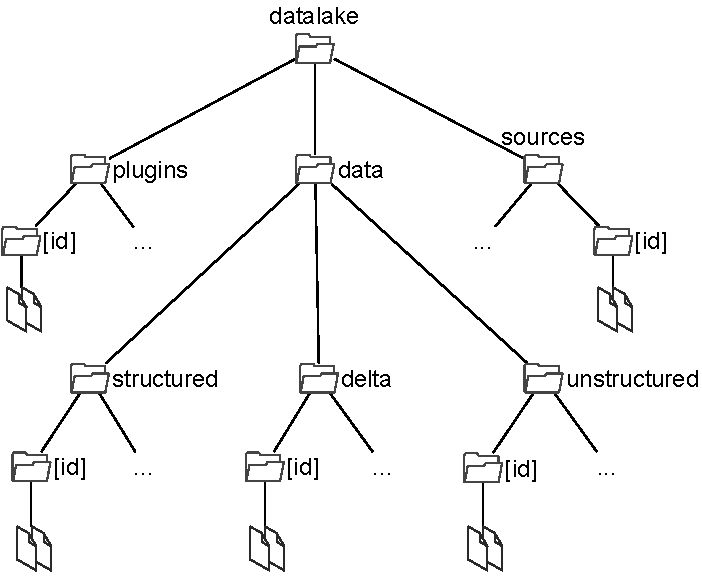
\includegraphics[width=.6\textwidth]{Grafiken/Umsetzung-Verzeichnisse.pdf}
    \caption{HDFS Verzeichnisstruktur}
    \label{fig:hdfs-folder}
\end{figure}